\section{High-Definition Multimedia Interface (HDMI)}
We chose HDMI to show the output result from the FPGA.
The HDMI cable can carry audio, Ethernet and other information in addition to the video stream itself, but only the video stream was utilized for this project.
Our implementation of HDMI was based on the Xilinx application note 495\cite{xapp495} and its reference design files. In our implementation it is possible to take an HDMI input, do convolution on the input and then transmit the result as HDMI output. As our PCB consists of two HDMI connectors, it is possible to do this. Another way is getting the image data from the MCU or directly from the camera through the FPC connector, do convolution and then send the result as HDMI output.

\subsection{Transition-Minimized Differential Signaling}
Transition-Minimized Differential Signaling(TMDS) is a standard used for transmitting video data over HDMI. HDMI uses it at the physical layer, and our implementation use the native TMDS I/O interface that is featured by the Spartan-6 FPGAs.
Four channels of serial data establish the HDMI video transmission. It has three channels for the RBG color information and one for the pixel data rate clock. Each pixel has a 24-bit color depth, with each color being 8 bits each. These are separately convertered into 10-bit symbols before being serialized and transmitted onto the TMDS data channels. It is this 10:1 serialization ratio that makes the bit rate 10x faster than the actual pixel rate. During the video transmission the pixel symbol is periodically interlaced with four distinct control tokens representing blanking intervals. These control tokens provide accurate video line scan(HSYNC) and frame update(VSYNC) information. Control tokens are also used to identify word boundaries for synchronization purposes.


The technology is based on twisted pairs of cables transferring data using a differential encoding.
This encoding uses two cables for each bit and inverts the voltage difference between the cables in a pair whenever the bit represented by the pair should change.
Notice that, for the same voltage, this doubles the distance between the high and low states compared to using only a single cable and ground.
The lack of a need for a common ground also eliminates problems related to ground offset

TMDS transfers 10 bits at a time using an encoding that minimizes the number of transitions required between each set of bits.

\subsubsection{TMDS transmitter}
\begin{figure}[h!]
    \centering
    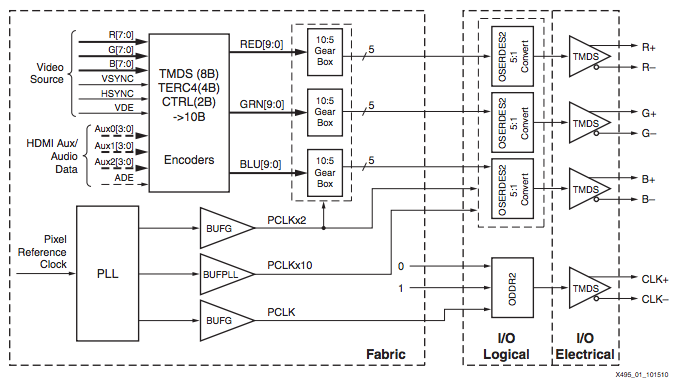
\includegraphics[scale= 0.7, angle = 90]{img/TMDStransmitterdesign.png}
    \caption{Overview of the TMDS transmitter design}
    \label{fig:TMDSTransmitter}
\end{figure}
The TMDS transmitter design can be seen in figure \ref{TMDSTransmitter}. Each color, VSYNC, HSYNC and VDE is sent to the TMDS encoders. In the verilog code this module is called dvi\_encoder. The output data is then serialized, using the serdes\_n\_to\_1 module. These serial bitstreams are then sent to the OBUFDS cores to produce the wanted output differential signals. The clock is produced using the PLL\_BASE module. The wanted pixel clock is then sent to the ODDR2 module, to get the wanted differential signal output.

\subsubsection{TMDS receiver}
\begin{figure}[h!]
    \centering
    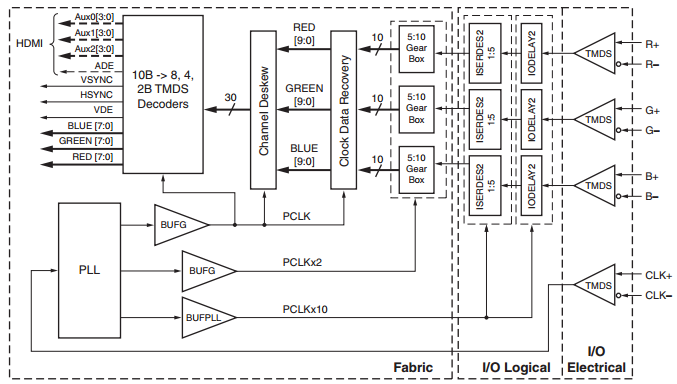
\includegraphics[scale= 0.7, angle = 90]{img/TMDSreceiverdesign.png}
    \caption{Overview of the TMDS receiver design}
    \label{fig:TMDSReceiver}
\end{figure}
The TMDS receiver needs to do clock and data recovery(CDR) to convert the serial data stream back into the 10-bit words and can be seen in figure \ref{TMDSReceiver}. This is done by using the incoming pixel clock to recover the bit sampling clock and then applying the bit clock to recover the serial data stream. Then skews among the three data channels are removed by using a channel deskew circuit. Then the 10-bit word is decoded into one of three possible formats:
* 8-bit video pixel data through the DVI or HDMI decoder
* 4-bit auxiliary data, i.e., information and audio frames through the HDMI decoder only
* 2-bit control data, e.g., the HSYNC and VSYNC through the DVI or HDMI decoder
